\documentclass[pdf]{beamer}
\usetheme{Copenhagen}
\usepackage{pgfgantt}
% Need to use LuaLatex to compile
\usepackage{emoji}
\usepackage{booktabs}
\usepackage{tikz}
\usepackage{fontawesome}
\usepackage{amsmath}
\usepackage{natbib}
\usetikzlibrary{angles,calc,intersections,quotes,arrows.meta,positioning}
\setemojifont{Apple Color Emoji}
\setbeamercovered{transparent}
\beamertemplatenavigationsymbolsempty
\setbeamertemplate{footline}[text line]{%
    \parbox{\linewidth}{\vspace*{-8pt}\hfill\hfill\insertframenumber\,/\,\inserttotalframenumber}}

\title{``$2^{\text{nd}}$'' Year PhD Seminar Presentation}

\author[Ananth Mahadevan]{Ananth Mahadevan}
\date{\today}

\begin{document}
\begin{frame}
    \titlepage
\end{frame}

\begin{frame}
    \frametitle{Quick Recap}
    \begin{itemize}
        \item \textbf{Masters:} Aalto University
        \item \textbf{Started:} Aug 2020 (contract) and Jan 2021 (study right) 
        \item \textbf{Supervisor:} Michael Mathioudakis
        \item \textbf{Research Group:} Algorithmic Data Science (ADS)
    \end{itemize}

    

\end{frame}

\begin{frame}[fragile]
    \frametitle{PhD Progress}
    \begin{ganttchart}[
        % hgrid,
        % vgrid,
        bar/.append style={fill=gray!50},
        time slot format=isodate-yearmonth,
        time slot unit=month,
        x unit=1.5mm,
        y unit chart=7mm,
        % y unit=1mm,
        progress label text={\pgfmathprintnumber[precision=0, verbatim]{#1}\%},
        % progress=today,
        today=2024-03,
        bar height=.5,
        group peaks width=1,
        group peaks height=0.4,
        rejected/.style={milestone/.append style={fill=red}},
        published/.style={milestone/.append style={fill=green}},
        review/.style={milestone/.append style={fill=yellow}},
        futurepublished/.style={milestone/.append style={fill=gray!50}},
        % bar top shift=.5
      ]{2020-01}{2024-12}
    \gantttitlecalendar{year} \\
      \ganttgroup[progress=today]{PhD}{2020-08}{2024-12}\\
      \ganttbar{Paper I}{2021-01}{2021-06} % Unlearning 
      \ganttmilestone[rejected]{}{2021-07} % VLDB-2022
      \ganttmilestone[rejected]{}{2022-02} % ECML_PKDD
      \ganttmilestone[published]{}{2022-04}\\ % MDPI-MAKE
      \ganttbar{Paper II}{2022-01}{2022-02} % JANE
      \ganttmilestone[rejected]{}{2022-03} % ANS extension 2022
      \ganttmilestone[published]{}{2022-06}\\
      \ganttbar{Paper III}{2020-08}{2020-09} % Sketching
      \ganttbar{}{2021-06}{2021-09} % Sketching
      \ganttbar{}{2022-03}{2022-05} % Sketching
      \ganttmilestone[published]{}{2022-09}\\ % CIKM 2022
      \ganttbar{Paper IV}{2022-05}{2023-02} % Reception Reader
      \ganttmilestone[published]{}{2023-04}\\ % JOHD 2023
      \ganttbar{Paper V}{2022-11}{2023-04} % Mandeville
      \ganttmilestone[published]{}{2023-12}\\ % JOHD 2023
      \ganttbar{Paper VI}{2021-11}{2022-12} % UpdateML
      \ganttmilestone[rejected]{}{2023-03} % ICML 2023
      \ganttmilestone[rejected]{}{2023-08} % EuroSys 2024
      \ganttmilestone[review]{}{2024-02}\\ % KBS 2024
      \ganttbar{Paper VII}{2023-06}{2024-02} % TextReuse Pipeline
      \ganttmilestone[futurepublished]{}{2024-04}\\ % KBS 2024

    \end{ganttchart}    

\end{frame}


\begin{frame}
    \frametitle{Papers}
    \begin{table}
        \centering
        \begin{tabular}{cccc}
            \toprule
            Number & One Word Title & Venue & Include in Thesis? \\
            \midrule
            I & Unlearning & MAKE 2022  & \emoji{check-mark-button}  \\
            II & JANE & Entropy 2022   &\emoji{check-mark-button} \\
            III & Sketching& CIKM 2022 & \emoji{man-shrugging-medium-skin-tone}\\
            IV & ReceptionReader& JOHD 2023 &  \emoji{man-shrugging-medium-skin-tone} \\
            V & Mandeville & DES 2023 & \emoji{man-shrugging-medium-skin-tone}\\
            VI & Retraining & KBS 2024 &  \emoji{check-mark-button} \\
            VII & TextReuse & VLDB 2024 & \emoji{check-mark-button} \\

            
        \end{tabular}
    \end{table}
\end{frame}


\begin{frame}
    \frametitle{Research Projects}
    % \begin{block}{\centering Broad Research Interests}
    %     \begin{center}
    %         Scalable Pipelines for Machine Learning and Data Science
    %     \end{center}
    % \end{block}

    Multiple Projects:
    \begin{enumerate}
        \item Maintaining ML models
        \begin{itemize}
            \item Paper I: Unlearning 
            \item Paper VI: Retraining
        \end{itemize}
        \item Analyzing Historical Documents 
        \begin{itemize}
            \item Paper IV: ReceptionReader
            \item Paper V: Mandeville
            \item Paper VII: TextReuse
        \end{itemize}
        \item Scaling and Evaluating Algorithms
        \begin{itemize}
            \item Paper II: JANE
            \item Paper III: Sketching 
            \item Paper VIII    ?: Diverse Sampling 
        \end{itemize}
    \end{enumerate}

\end{frame}


\begin{frame}
    \frametitle{Maintaining ML models}

    \begin{block}{\centering Research Question}
        \centering
        How to update a trained ML model when the data changes?
    \end{block}

    \begin{enumerate}
        \item Machine Unlearning 
        \begin{itemize}
            \item Training data is deleted/removed
            \item Update model parameters to forget information
        \end{itemize}
        \item Cost-Aware Retraining
        \begin{itemize}
            \item Streams drift over time
            \item Data and Queries are present
            \item Retraining consumes resources
            \item When is it worth retraining?
        \end{itemize}
    \end{enumerate}
\end{frame}


\begin{frame}
    \frametitle{Analyzing Historical Documents}
    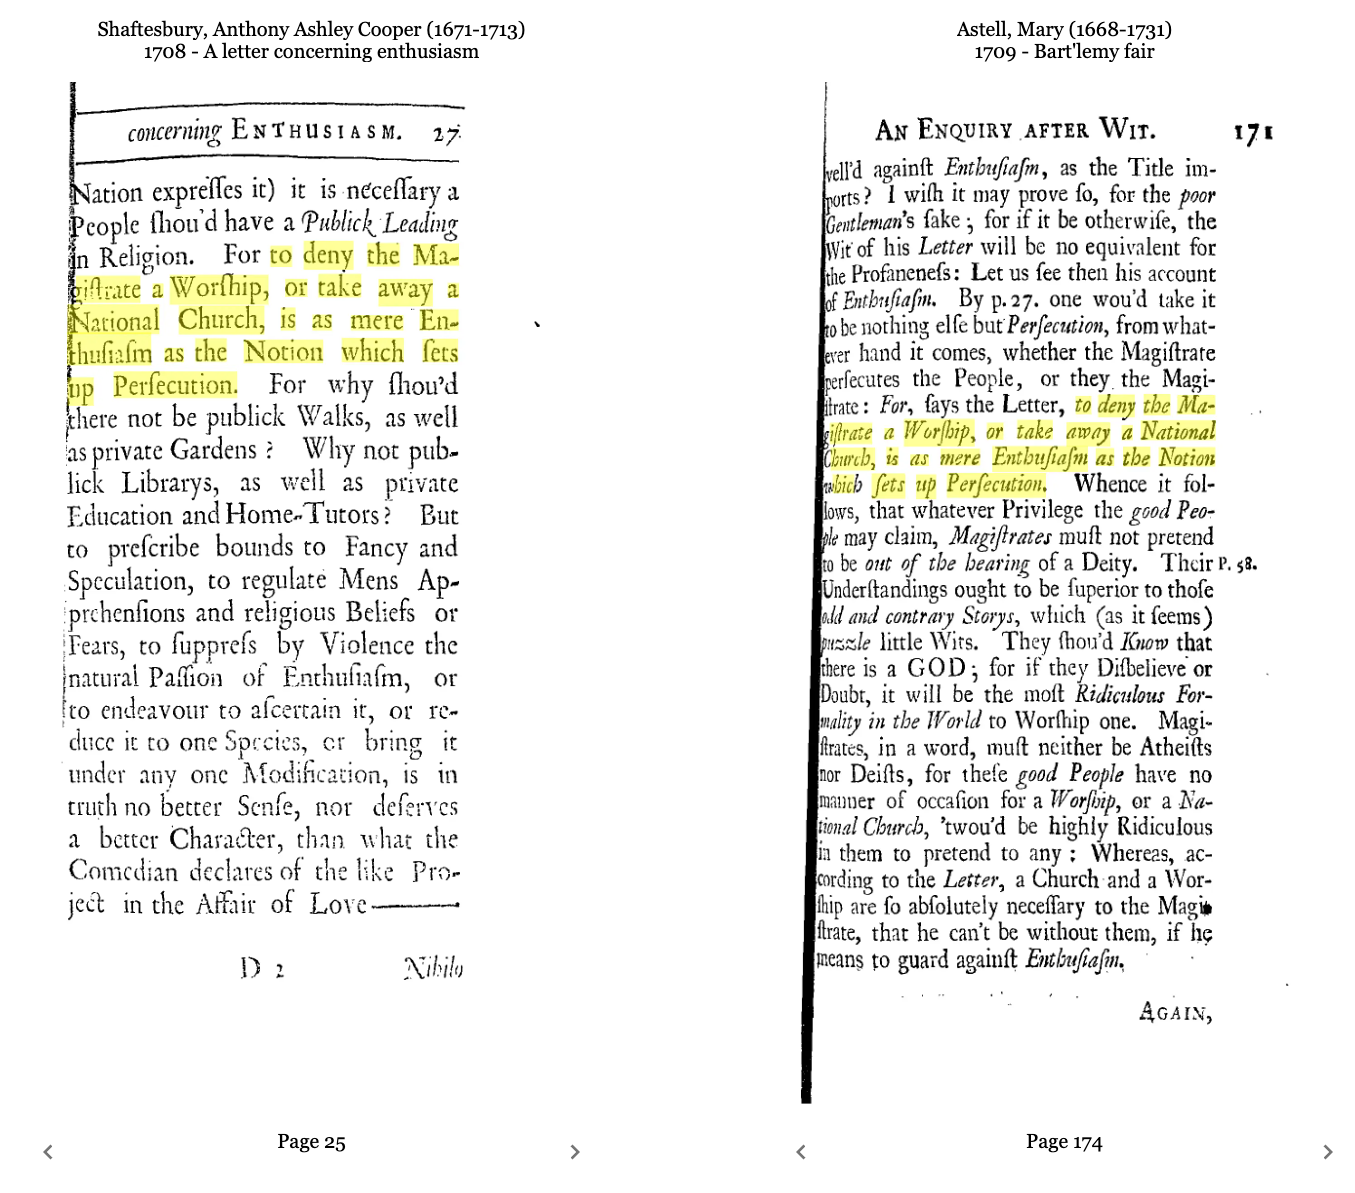
\includegraphics[width=\textwidth]{figs/Reception-Reader-Example.png}
    

\end{frame}

\begin{frame}[fragile]
    \frametitle{Analyzing Historical Documents}


        However, OCR texts are very noisy
        \begin{block}{Document 1 string}
            \footnotesize
            \begin{verbatim}
            to deny the Ma-
            tifl:ate a Worflip, or take away a
            hational Church, is as mere En-
            Ihufiafin as the Notion which sets
            uip Persecution    
            \end{verbatim}
        \end{block}    
        \begin{block}{Document 2 string}
            \footnotesize
            \begin{verbatim}
            , to deny the Ala-
            inrate a ITorftip, or take awvay a National
            'uircb, is as mere Entnztfiafm as the Notion
            .bic fJets tup Persecution. W
            \end{verbatim}
        \end{block}    
        How?
        \begin{itemize}
            \item Use BLAST to do fuzzy alignment
        \end{itemize}
\end{frame}

\begin{frame}[fragile]
    \frametitle{Pre-Processing Pipeline}
    \scalebox{0.5}{
    \newcommand\file[2]{%
    \begin{scope}[xshift=#1cm,yshift=#2cm]
      \draw[gray,thick] (0,0) -- (0,1.5) -- (0.7,1.5) -- (0.7,1.1) -- (1,1.1) -- (1,0) -- cycle;
      \draw[gray,thick] (0.7,1.5) -- (1,1.1);
      \foreach \y in {0.2,0.3,...,1.1}{
         \draw[thick] (0.2,\y) -- (0.8,\y);
         }
      \foreach \y in {1.1,1.2,...,1.4}{
         \draw[thick] (0.2,\y) -- (0.65,\y);
         }
        %  \draw[thick] (0.2,0.8) -- (0.6,0.8);
        %  \draw[thick] (0.2,1) -- (0.6,1);
    \end{scope}
}

% https://tex.stackexchange.com/questions/126161/how-can-i-draw-a-tikz-element-multiple-times-against-a-shaded-background
% \pgfkeys{/tikz/.cd,
%    at/.initial={(0,0)},
%    at/.get=\coordpos,
%    at/.store in=\coordpos,   
%    my tree/.code={
%     \draw[gray] \coordpos -- +(0,1.2) -- +(0.7,1.2) -- +(0.7,0.8) -- +(1,0.8) -- +(1,0) -- cycle;
%     \draw[gray] +(0.7,1.2) -- +(1,0.8);
%     \foreach \y in {0.2,0.4,0.6}{
%         \draw (0.2,\y) -- (0.8,\y);
%         \draw (0.2,0.8) -- (0.6,0.8);
%         \draw (0.2,1) -- (0.6,1);
%     }
%    }
% }
\begin{tikzpicture}
    \tikzset{
      piece/.style 2 args={red,draw,thick,rectangle,anchor=south west,minimum width=#1,minimum height=#2},
      defrag piece/.style 2 args={blue,draw,thick,rectangle,anchor=south west,minimum width=#1,minimum height=#2},
      source piece/.style 2 args={orange,draw,very thick,rectangle,anchor=south west,minimum width=#1,minimum height=#2},
      destination piece/.style 2 args={green!50!black,draw,very thick,rectangle,anchor=south west,minimum width=#1,minimum height=#2},
      reuse/.style={red,-,very thick},
      defrag reuse/.style={blue,-,very thick},
      reception/.style={black,-{Latex[scale=1]},very thick},
      cluster/.style={violet,-,very thick,rounded corners=10pt,rectangle}
    }
    \begin{scope}[local bounding box=scope1]
    % \draw [help lines] (0,-2) grid (4,4);
    \file{0}{0}
    \node at (0.5,1.65) {A};
    \node[piece={0.8cm}{0.4cm}] at (0.1,0.1) (tr11) {};
    \node[piece={0.54cm}{0.4cm}] at (0.1,1.1) (tr12) {};
    \file{1.5}{1.5}
    \node at (2,3.15) {B};
    \node[piece={0.8cm}{0.4cm}] at (1.55,1.55) (tr21) {};
    \node[piece={0.78cm}{0.5cm}] at (1.64,1.63) (tr22) {};
    \file{3}{0}
    \node at (3.5,1.65) {C};
    \node[piece={0.54cm}{0.4cm}] at (3.1,0.95) (tr31) {};
    \node[piece={0.8cm}{0.4cm}] at (3.1,0.1) (tr32) {};
    \file{1.5}{-1.5}
    \node at (2,0.15) {D};
    \node[piece={0.8cm}{0.4cm}] at (1.55,-1.45) (tr41) {};
    \node[piece={0.78cm}{0.5cm}] at (1.63,-1.36) (tr42) {};
    \draw[reuse] (tr12.east) -- (tr21.west);
    \draw[reuse] (tr11.east) -- (tr41.west);
    \draw[reuse] (tr42.east) -- (tr32.west);
    \draw[reuse] (tr22.east) -- (tr31.west);
    % \node at (2,-1.68) {};
    % \matrix [below left] at (current bounding box.north east) {
    % \node [piece={0.5cm}{0.1cm},label=right:Piece] {};\\
    % \node[reuse,inner sep=0,minimum width=4mm,draw,anchor= south west,label=right:Text Reuse] at ++(1mm,0) {};\\
    % };
    \end{scope}

    \begin{scope}[local bounding box=scope2,shift={(scope1.base east)},xshift=3cm]
    % \draw [help lines] (0,-2) grid (4,4);
    \file{0}{0}
    \node at (0.5,1.65) {A};
    \node[defrag piece={0.8cm}{0.4cm}] at (0.1,0.1) (tr11) {};
    \node[defrag piece={0.54cm}{0.4cm}] at (0.1,1.1) (tr12) {};
    \file{1.5}{1.5}
    \node at (2,3.15) {B};
    \node[defrag piece={0.8cm}{0.54cm}] at (1.58,1.6) (tr21) {};
    \file{3}{0}
    \node at (3.5,1.65) {C};
    \node[defrag piece={0.54cm}{0.4cm}] at (3.1,0.95) (tr31) {};
    \node[defrag piece={0.8cm}{0.4cm}] at (3.1,0.1) (tr32) {};
    \file{1.5}{-1.5}
    \node at (2,0.15) {D};
    \node[defrag piece={0.8cm}{0.54cm}] at (1.6,-1.4) (tr41) {};
    \draw[defrag reuse] (tr12.east) -- (tr21.west);
    \draw[defrag reuse] (tr11.east) -- (tr41.west);
    \draw[defrag reuse] (tr41.east) -- (tr32.west);
    \draw[defrag reuse] (tr21.east) -- (tr31.west);
    
    \draw[cluster] (-0.1,0.9) rectangle (4,2.3) ;
    \draw[cluster] (-0.1,0.6) rectangle (4.2,-1.5) ;
    % \draw[cluster] plot [smooth cycle] coordinates{(0.1,1) (3.8,0.95) (3.5,2) (2,2.25) (0.6,2) };
    % \draw[cluster] plot [smooth cycle] coordinates{(0.0,0.6)  (4,0.6) (3.5,-1) (2,-1.75) (0.55,-1)};
    \end{scope}

    \begin{scope}[local bounding box=scope3,shift={(scope2.base east)},xshift=3cm]
      % \draw [help lines] (0,-2) grid (4,4);
      \file{0}{0}
      \node at (0.5,1.65) {A};
      \node[source piece={0.8cm}{0.4cm}] at (0.1,0.1) (tr11) {};
      \node[destination piece={0.54cm}{0.4cm}] at (0.1,1.1) (tr12) {};
      \file{1.5}{1.5}
      \node at (2,3.15) {B};
      \node[source piece={0.8cm}{0.54cm}] at (1.58,1.6) (tr21) {};
      \file{3}{0}
      \node at (3.5,1.65) {C};
      \node[destination piece={0.54cm}{0.4cm}] at (3.1,0.95) (tr31) {};
      \node[destination piece={0.8cm}{0.4cm}] at (3.1,0.1) (tr32) {};
      \file{1.5}{-1.5}
      \node at (2,0.15) {D};
      \node[destination piece={0.8cm}{0.54cm}] at (1.6,-1.4) (tr41) {};
      \draw[reception] (tr11.east) -- (tr41.west);
      \draw[reception] (tr11.east) -- (tr32.west);

      \draw[reception] (tr21.west) -- (tr12.east);
      \draw[reception] (tr21.east) -- (tr31.west);
        
      \draw[cluster] (-0.1,0.9) rectangle (4,2.3) ;
      \draw[cluster] (-0.1,0.6) rectangle (4.2,-1.5) ;
    %   \draw[cluster] plot [smooth cycle] coordinates{(0.1,1) (3.8,0.95) (3.5,2) (2,2.25) (0.6,2) };
    %   \draw[cluster] plot [smooth cycle] coordinates{(0.0,0.6)  (4,0.6) (3.5,-1) (2,-1.75) (0.55,-1)};
      \end{scope}

      \draw [->,black,very thick] ($(scope1.east)!0.1!(scope2.west)$) -- ($(scope1.east)!0.9!(scope2.west)$)  node[midway,above]{Defragment} node[midway,below] {\& Cluster};
      \draw [->,black,very thick] ($(scope2.east)!0.1!(scope3.west)$) -- ($(scope2.east)!0.9!(scope3.west)$)  node[midway,above]{Identify Sources} node[midway,below] {\& Destinations};

    \matrix [draw,matrix anchor = south,yshift=5mm] at ($(scope1.north west)!0.5!(scope3.north east)$) {
    \node [inner sep=0,label=right:Doc,anchor=south west] at (0,-0.5mm){\faFileTextO}; & 
    \node [piece={0.5cm}{0.1cm},label=right:Piece] {}; & 
    \node[reuse,inner sep=0,minimum width=4mm,draw,anchor=south west,label=right:Text Reuse] at ++(0,1mm) {}; & 
    \node [defrag piece={0.5cm}{0.1cm},label=right:Defrag Piece] {}; & 
    \node[defrag reuse,inner sep=0,minimum width=4mm,draw,anchor= south west,label=right:Defrag Text Reuse] at ++(0,1mm) {}; & 
    \node[draw,cluster,anchor=south west,minimum width=0.5cm,minimum height=0.1cm,rounded corners=2pt,rectangle,label=right:Cluster] {};& 
    \node [source piece={0.5cm}{0.1cm},label=right:Source Piece] {}; & 
    \node [destination piece={0.5cm}{0.1cm},label=right:Destination Piece] {}; & 
    \draw[reception] (0,1mm) -- (5mm,1mm) node[inner sep =0,minimum size =0,right,anchor=west] {Reception};
    \\
    };
\end{tikzpicture}

%

% \node[label=below:Document,inner sep=0,minimum size =0] {\faFileTextO}; & 
% \node [piece={0.5cm}{0.3cm},anchor=center,label=below:Piece] {}; & 
% \draw[reuse] (0,0mm) -- (5mm,0mm) node[inner sep =0,minimum size =0,midway,below=4mm,anchor=center,black] {Text Reuse};&
% \node [defrag piece={0.5cm}{0.3cm},anchor=center,label=below:Defrag Piece] {};& 
% \draw[defrag reuse] (0,0mm) -- (5mm,0mm) node[inner sep =0,minimum size =0,midway,below=4mm,anchor=center,black] {Defrag Text Reuse};&
% \draw[cluster] (0,0mm) -- +(5mm,0mm) node[inner sep =0,minimum size =0,midway,below=3.6mm,anchor=center,black] {~Cluster};&
% \node [source piece={0.5cm}{0.3cm},anchor=center,label=below:Source Piece] {}; & 
% \node [destination piece={0.5cm}{0.3cm},anchor=center,label=below:Destination Piece] {}; & 
% \draw[reception] (0,0mm) -- +(5mm,0mm) node[inner sep =0,minimum size =0,midway,below=4mm,anchor=center] {Reception};
% \\
    }
    \begin{itemize}
        \item Clean up BLAST hits for downstream tasks
        \item Implemented in Apache Spark
        \item Scales up to {\bf 6.31 billion} pairs of reuses
    \end{itemize}
\end{frame}

\begin{frame}
    \frametitle{Related Publications}

    \begin{enumerate}
        \item Paper IV: \citet{Rosson-2023}
        \begin{itemize}
            \item \emph{Reception reader: Exploring text reuse in early modern british publications}
            \item Front-end user interface for browsing reuses
        \end{itemize}
        \item Paper V: \citet{des6}
        \begin{itemize}
            \item \emph{A Comparative text similarity analysis of the works of Bernard Mandeville}
            \item Study using the data and interfaces from \cite{Rosson-2023}
        \end{itemize}
        \item Paper VI: \citet{mahadevan2024optimizing}
        \begin{itemize}
            \item \emph{Optimizing a Data Science System for Text Reuse Analysis}
            \item Studies design choices for the optimal performance of the system
        \end{itemize}
    \end{enumerate}


\end{frame}
\begin{frame}
    \frametitle{Scalability and Robustness}
\end{frame}

\begin{frame}[allowframebreaks]
    \frametitle{References}
    \bibliographystyle{plainnat}
    \bibliography{references.bib}
  \end{frame}

\end{document}